
\chapter{Analyse et spécification des besoins}
\label{chap:Analyse et spécification des besoins}



Dans ce chapitre, nous abordons l’étape d’analyse et spécification des besoins pour notre projet. Ainsi nous présentons en premier temps les acteurs ainsi que les exigences fonctionnelles et non-fonctionnelles du projet. Puis, nous utilisons les diagrammes de cas d’utilisations avec leurs descriptions textuelles pour décrire les scénarios possibles. Cela nous permettra de guider le développement du système de manière efficace et d’assurer sa conformité aux exigences.

\pagebreak

\section{Étude de l’existant}

Reconnu depuis 30 ans comme un partenaire privilégié du monde de l'éducation, 4D accompagne les directeurs d'établissements, les enseignants, les chercheurs et les responsables administratifs dans la réussite de leurs parcours. L'entreprise offre deux types de formation : la formation sur mesure et la formation standard. La formation sur mesure est adaptée spécifiquement aux besoins individuels de l'apprenant, permettant une personnalisation maximale du contenu et des méthodes d'enseignement. En revanche, la formation standard est une offre prédéfinie par l'entreprise, accessible à tout apprenant intéressé. Ces formations peuvent être suivies en ligne, à travers des plateformes telles que Zoom ou Google Meet, ou en présentiel, selon les modalités fixées par l'entreprise.

Avant la pandémie de COVID-19, la plupart des formations se déroulaient en mode présentiel. Cependant, avec la montée en puissance du travail à distance, les entreprises ont découvert qu'il était possible de réaliser de nombreuses tâches en ligne. En conséquence, 4D a décidé de migrer vers les formations à distance. Cependant, l'utilisation des outils de visioconférences présente plusieurs limitations. La gestion des formations nécessite un grand effort manuel, et les formations ne sont pas regroupées dans un seul endroit où l'utilisateur peut consulter et choisir ce qui est adéquat pour ses besoins. la formation à travers ces outils n'est pas très productif pour l'apprenant. Il est donc nécessaire de trouver une solution plus efficace pour gérer et proposer les formations en ligne

\section{Spécification des exigences}

Cette phase de l’application vise à définir la frontière fonctionnelle entre le système et son environnement. Pour affiner les objectifs définis dans le contexte général du projet, il est essentiel de répondre à deux questions principales : Quels sont les utilisateurs du système ? Qu'attendent-ils de ce système ?

Pour trouver la réponse, nous avons opté pour la démarche suivante : 

- Définir les acteurs du système. 

- Lister ce que doit offrir le système à son utilisateur.


\subsection{Etude fonctionnelle et non fonctionnelle}
\subsubsection{Identification des acteurs}

Un acteur représente l’abstraction d’un rôle joué par des entités externes qui
interagissent directement avec le système étudié. Un acteur peut consulter et/ou
modifier directement l’état du système, en émettant et/ou en recevant des messages
susceptibles d'être porteur de données.

\begin{table}[htbp]
    \centering
    \begin{tabular}{|m{5cm}|m{10cm}|}
        \hline
        \textbf{Acteur} & \textbf{Rôle dans l'application} \\
        \hline
        Administrateur & Responsable de la gestion technique et opérationnelle de l'application, de la gestion des comptes des utilisateurs (Formateurs et Apprenants), de la sécurité des données et du support technique. Ainsi la création, gestion et mise à jour des cours. \\
        \hline
        Apprenant & Utilisateur principal de la plateforme, pouvant accéder aux cours, suivre les chapitres de formation, évaluer les contenus. \\
        \hline
    \end{tabular}
    \caption{Acteurs de l'application}
    \label{tab:roles}
\end{table}

\subsubsection{Identification des fonctionnalités}

\subsubsection*{Authentification}

C’est l’étape primordiale pour toutes les fonctionnalités. Il s’agit de saisir un identifiant (email ou nom d'utilisateur) et un mot de passe puis de valider pour pouvoir exploiter les autres services.

\subsubsection*{Apprenant}
\begin{itemize}
    \item[$\bullet$] \textbf{Gestion des Abonnements:} Permettre aux apprenants de payer un abonnement pour accéder aux formations.
    \item[$\bullet$] \textbf{Gestion des Formations pour les Apprenants:}
    \begin{itemize}
        \item \textit{S'inscrire à une formation:} Permettre aux apprenants de s'inscrire à une formation après s'être authentifiés et avoir payé l'abonnement si nécessaire.
        \item \textit{ Consulter une formation:} Permettre aux apprenants de consulter les détails d'une formation à laquelle ils sont inscrits.
        \item \textit{Évaluer une formation:} Permettre aux apprenants d'évaluer une formation après l'avoir suivie.
        \item \textit{ Chercher une formation:} Permettre aux apprenants de rechercher les formations disponibles sur la plateforme.
        \item \textit{Consulter le profil d'un formateur:} Permettre aux apprenants de consulter les profils des formateurs sur la plateforme.
    \end{itemize}
    \item[$\bullet$] \textbf{Gestion de Profil:}
    \begin{itemize}
        \item  Modifier son profil: Permettre aux apprenants de modifier leurs informations personnelles sur leur profil.
    \end{itemize}
\end{itemize}
    
\subsubsection*{Administrateur}
\begin{itemize}
    \item[$\bullet$] \textbf{Gestion des Formations:}
    \begin{itemize}
        \item  Ajouter une formation: Permettre aux administrateurs d'ajouter une nouvelle formation sur la plateforme.
        \item  Modifier une formation: Permettre aux administrateurs de modifier une formation existante.
        \item  Supprimer une formation: Permettre aux administrateurs de supprimer une formation existante.
    \end{itemize}
    \item[$\bullet$] \textbf{Gestion des Apprenants:}
    \begin{itemize}
        \item  Ajouter un apprenant: Permettre aux administrateurs d'ajouter un nouveau apprenant sur la plateforme.
        \item  Modifier un apprenant: Permettre aux administrateurs de modifier un apprenant existant.
        \item  Supprimer un apprenant: Permettre aux administrateurs de supprimer un apprenant existant.
    \end{itemize}
    \item[$\bullet$] \textbf{Gestion des Formateurs:}
    \begin{itemize}
        \item  Ajouter un formateur: Permettre aux administrateurs d'ajouter un nouveau formateur sur la plateforme.
        \item  Modifier un formateur: Permettre aux administrateurs de modifier un formateur existant.
        \item  Supprimer un formateur: Permettre aux administrateurs de supprimer un formateur existant.
    \end{itemize}
    \item[$\bullet$] \textbf{Gestion des Statistiques:}
    \begin{itemize}
        \item  Consultation les statistiques: Offrir aux administrateurs la possibilité d'accéder à une interface dédiée où ils peuvent consulter diverses statistiques de la plateforme comme le nombre des apprenants et des formateurs.
    \end{itemize}
\end{itemize}


\subsubsection{Diagramme de cas d’utilisation}

Les diagrammes des cas d'utilisation décrivent les fonctions générales et la portée d'un système. Ces diagrammes identifient également les interactions entre le système et ses acteurs.

Nous synthétisons dans ce paragraphe tout ce qui a été dit dans la phase d’analyse. Nous présentons le diagramme de cas d’utilisation de notre application et introduisons les cas d’utilisation qui la composent.

\begin{figure}[H]
    \centering
    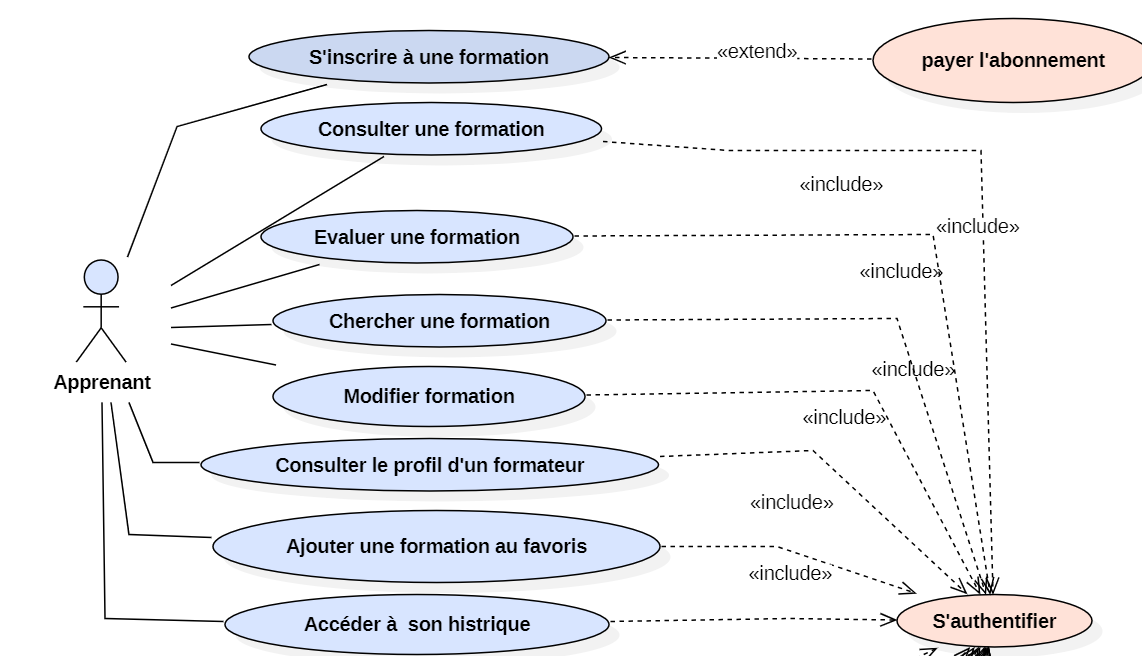
\includegraphics[width=15cm]{Figures/apprenant.PNG}
    \caption{Diagramme de cas d’utilisation d'apprenant}
\end{figure}

\begin{figure}[H]
    \centering
    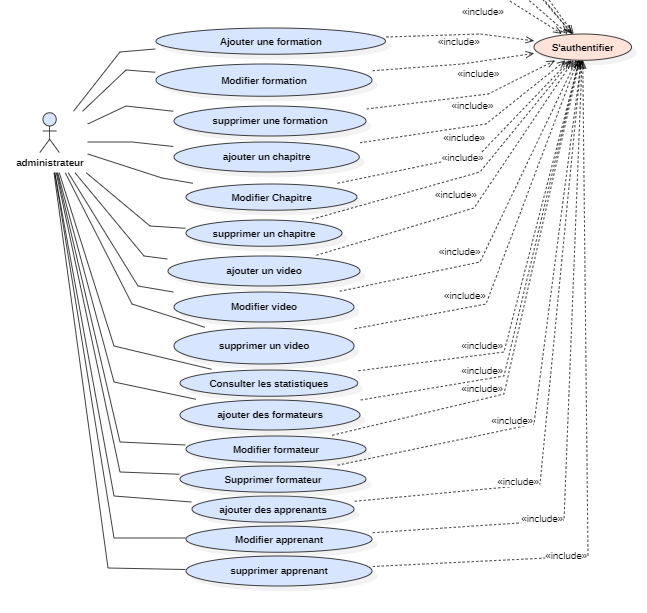
\includegraphics[width=13cm]{Figures/administrateur.PNG}
    \caption{Diagramme de cas d’utilisation d'administrateur}
\end{figure}

\subsubsection{Description textuelle de cas d’utilisation}

\begin{minipage}{\textwidth}
\begin{table}[H]
\centering
\begin{tabular}{| m{8cm} | m{8cm} |}
\hline
\multicolumn{2}{|c|}{\textbf{UC 1:} Payer l'abonnement d'une formation} \\ \hline
\textbf{Acteurs} & Apprenant \\ \hline
\textbf{But} & Permettre à un apprenant d'accéder à une formation disponible sur la plateforme et voir les vidéos \\ \hline
\textbf{Préconditions} & \textbf{Postconditions} \\ \hline
- S'authentifier. & - Voir les vidéos \\ \hline
\textbf{Scénario Principal} & \textbf{Scénario Alternatif} \\ \hline
\begin{enumerate}
    \item S'authentifier.
    \item Naviguer vers la page de la formation.
    \item Choisir la formation.
    \item Cliquer sur "S'inscrire".
    \item Effectuer le paiement.
    \item vérifier si le paiement est autorisé.
    \item Redirection vers la page de confirmation de paiement.
\end{enumerate} & 
\begin{enumerate}
    \item S'authentifier.
    \item Naviguer vers la page de la formation.
    \item Choisir la formation.
    \item Cliquer sur "S'inscrire".
    \item Effectuer le paiement.
    \item vérifier si le paiement est autorisé.
    \item Redirection vers la page d’erreur.
\end{enumerate} \\ \hline
\end{tabular}
\caption{Description Textuelle du Cas d'Utilisation "Payer l'abonnement d'une formation"}
\label{tab:use_case_description_1}
\end{table}
\end{minipage}

\newpage

\begin{minipage}{\textwidth}
\begin{table}[H]
\centering
\begin{tabular}{| m{8cm} | m{8cm} |}
\hline
\multicolumn{2}{|c|}{\textbf{UC 2:} Ajouter une formation} \\ \hline
\textbf{Acteurs} & Administrateur \\ \hline
\textbf{But} & Permettre à un administrateur d'ajouter une formation à la plateforme avec ses chapitres et ses vidéos \\ \hline
\textbf{Préconditions} & \textbf{Postconditions} \\ \hline
- S'authentifier. & Formation ajoutée \\ \hline
\textbf{Scénario Principal} & \textbf{Scénario Alternatif} \\ \hline
\begin{enumerate}
    \item S'authentifier.
    \item Naviguer vers la page d'ajout de formation.
    \item Remplir les informations nécessaires pour la formation.
    \item Ajouter les chapitres.
    \item Ajouter les vidéos.
    \item Cliquer sur le bouton "Enregistrer".
    \item Un message de confirmation est affiché.
\end{enumerate} & 
\begin{enumerate}
    \item S'authentifier.
    \item Naviguer vers la page d'ajout de formation.
    \item Remplir les informations nécessaires pour la formation.
    \item Ajouter les chapitres.
    \item Ajouter les vidéos.
    \item Cliquer sur le bouton "Enregistrer".
    \item Un message d'erreur spécifiant les champs incorrects ou manquants est affiché.
\end{enumerate} \\ \hline
\end{tabular}
\caption{Description Textuelle du Cas d'Utilisation "Ajouter une formation"}
\label{tab:use_case_description_2}
\end{table}
\end{minipage}

\newpage

\begin{minipage}{\textwidth}
\begin{table}[H]
\centering
\begin{tabular}{| m{8cm} | m{8cm} |}
\hline
\multicolumn{2}{|c|}{\textbf{UC 3:} Ajouter un chapitre} \\ \hline
\textbf{Acteurs} & Administrateur \\ \hline
\textbf{But} & Permettre à un administrateur d'ajouter un chapitre à une formation existante \\ \hline
\textbf{Préconditions} & \textbf{Postconditions} \\ \hline
- S'authentifier. & Chapitre ajouté \\ \hline
\textbf{Scénario Principal} & \textbf{Scénario Alternatif} \\ \hline
\begin{enumerate}
    \item S'authentifier.
    \item Naviguer vers la page des formations.
    \item Choisir une formation.
    \item Remplir les informations nécessaires pour le chapitre.
    \item Ajouter les vidéos.
    \item Cliquer sur le bouton "Enregistrer".
    \item Afficher un message de confirmation.
\end{enumerate} & 
\begin{enumerate}
    \item S'authentifier.
    \item Naviguer vers la page des formations.
    \item Choisir une formation.
    \item Remplir les informations nécessaires pour le chapitre.
    \item Ajouter les vidéos.
    \item Cliquer sur le bouton "Enregistrer".
    \item Afficher un message d'erreur spécifiant les champs incorrects ou manquants.
\end{enumerate} \\ \hline
\end{tabular}
\caption{Description Textuelle du Cas d'Utilisation "Ajouter un chapitre"}
\label{tab:use_case_description_3}
\end{table}
\end{minipage}

\newpage

\begin{minipage}{\textwidth}
\begin{table}[H]
\centering
\begin{tabular}{| m{8cm} | m{8cm} |}
\hline
\multicolumn{2}{|c|}{\textbf{UC 4:} Ajouter un apprenant} \\ \hline
\textbf{Acteurs} & Administrateur \\ \hline
\textbf{But} & Permettre à un administrateur d'ajouter un apprenant pour qu'il puisse s'authentifier à la plateforme. \\ \hline
\textbf{Préconditions} & \textbf{Postconditions} \\ \hline
- S'authentifier. & Apprenant ajouté \\ \hline
\textbf{Scénario Principal} & \textbf{Scénario Alternatif} \\ \hline
\begin{enumerate}
    \item S'authentifier.
    \item Naviguer vers la page des apprenants.
    \item Remplir les informations nécessaires pour l'apprenant.
    \item Cliquer sur le bouton "Enregistrer".
    \item Afficher un message de confirmation.
\end{enumerate} & 
\begin{enumerate}
    \item S'authentifier.
    \item Naviguer vers la page des apprenants.
    \item Remplir les informations nécessaires pour l'apprenant.
    \item Cliquer sur le bouton "Enregistrer".
    \item Afficher Un message d'erreur spécifiant les champs incorrects ou manquants.
\end{enumerate} \\ \hline
\end{tabular}
\caption{Description Textuelle du Cas d'Utilisation "Ajouter un apprenant"}
\label{tab:use_case_description_4}
\end{table}
\end{minipage}




\subsubsection{Diagramme de séquence de système}

\subsubsection*{Diagramme de séquence de l’authentification}

L’authentification est l’étape primordiale pour toutes les fonctionnalités. L'interaction débute par l’utilisateur qui saisit ses informations d'authentification (username et mot de passe) et les envoie au système.
Dans le premier cas, le système transmet ces informations à sa base de données pour vérification. Si les informations sont correctes, le système redirige l'utilisateur vers la page d'accueil.
Dans le deuxième cas, si les informations d'authentification sont incorrectes, la base de données envoie une réponse négative au système. Le système informe alors l'utilisateur que les informations saisies sont incorrectes, et il est redirigé vers la page d'authentification pour qu'il puisse réessayer.


\begin{figure}[H]
    \centering
    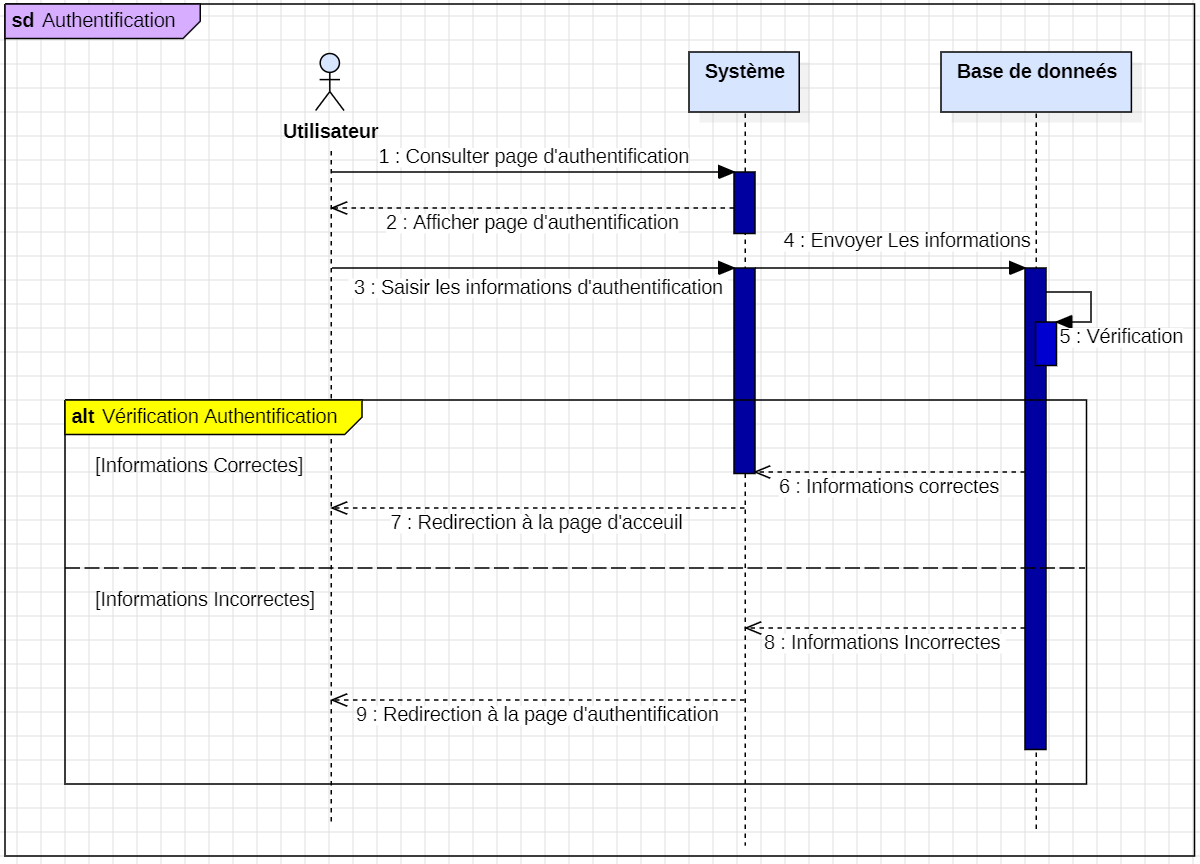
\includegraphics[width=19cm]{Figures/diagrammeDeSequenceAuthentification.png}
    \caption{Diagramme De Séquence De l'Authentification}
\end{figure}

\subsubsection*{Diagramme de séquence d’ajouter une formation}

Ce diagramme montre comment un administrateur ajoute une formation. L'administrateur clique sur "ajouter formation", un formulaire s'affiche, et les informations sont saisies. Le processus se poursuit avec l'ajout de chapitres et de vidéos, l'importation des vidéos et l'envoi des données pour la création de la formation. Une notification est affichée pour indiquer si la création a réussi ou échoué.

\begin{figure}[H]
    \centering
    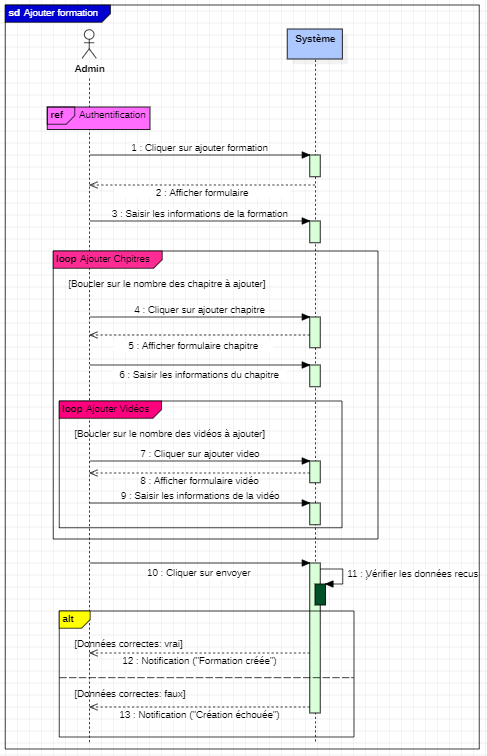
\includegraphics[width=15cm]{Figures/diagrammeDeSequenceCreerCourse.PNG}
    \caption{Diagramme De Séquence d'Ajouter Une Formation}
\end{figure}

\subsubsection*{Diagramme de séquence d'ajouter un formateur}

Le diagramme de séquence montre le processus par lequel un administrateur ajoute un formateur. L'administrateur clique sur "ajouter formateur" et le système affiche un formulaire à remplir. Après la soumission du formulaire, le système envoie une requête à la base de données pour créer le formateur. Si la création réussit, le système notifie l'administrateur que le formateur a été ajouté avec succès. En cas d'échec, une notification d'échec est envoyée.

\begin{figure}[H]
    \centering
    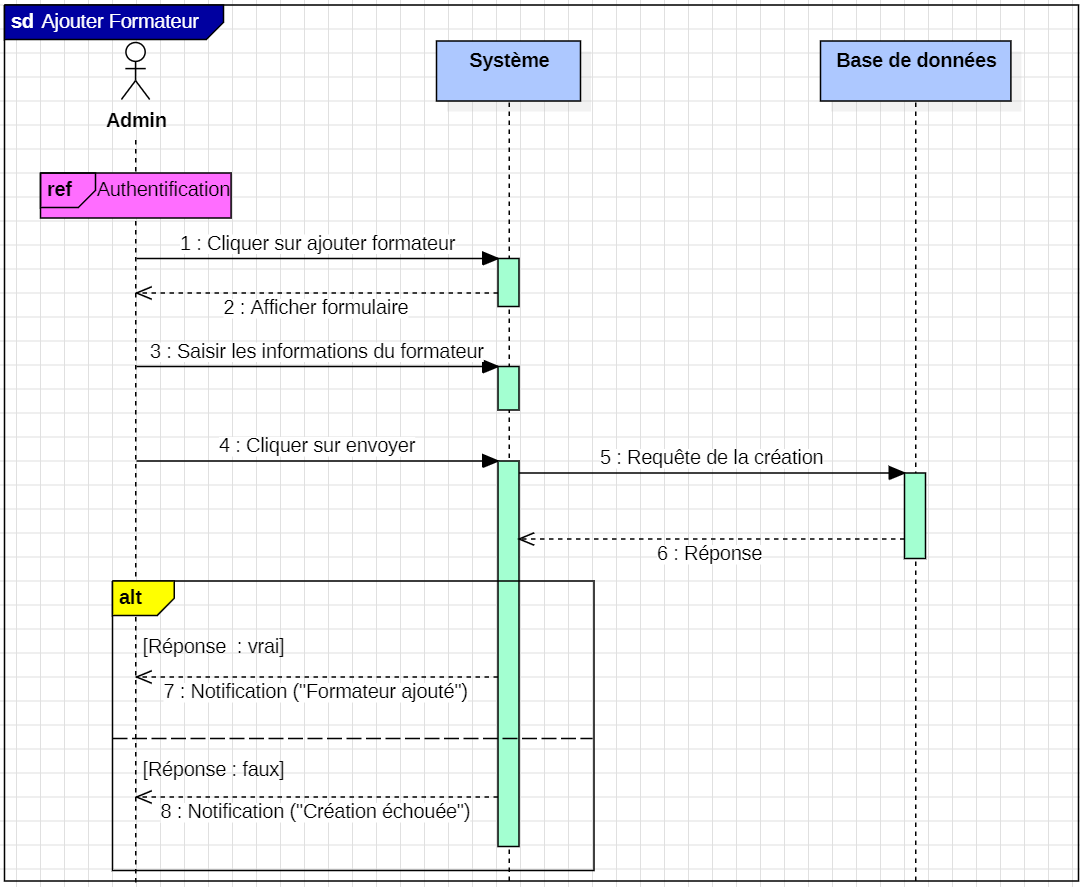
\includegraphics[width=17cm]{Figures/diagrammeDeSequenceAddAuthor.PNG}
    \caption{Diagramme De Séquence D'ajouter Formateur}
\end{figure}


\subsection{Exigences non-fonctionnelles}


Ce sont les besoins qui permettent d’améliorer la qualité des services de la plateforme comme la convivialité et l’ergonomie des interfaces et l’amélioration du temps de réponse. Parmi ces besoins, on cite :

\begin{itemize}
    \item[$\bullet$] \textbf{Convivialité:} La future application doit être facile à utiliser. En effet, les interfaces utilisateur doivent être conviviales c’est-à-dire simples, ergonomiques et adaptées à l’utilisateur.
    \item[$\bullet$] \textbf{Maintenabilité:} Toute architecture est exposée à des évolutions au niveau de la technologie d’implémentation. La solution doit avoir un grand niveau d’abstraction pour faciliter les nouvelles implémentations.
    \item[$\bullet$] \textbf{Performance:} Le temps de réponse doit être le plus court possible.
    \item[$\bullet$] \textbf{Disponibilité:} Lorsque n’importe quel utilisateur désire consulter la plateforme, elle doit être disponible.
    \item[$\bullet$] \textbf{Sécurité:} La plateforme doit protéger les données personnelles des utilisateurs, garantir l'intégrité des cours et du contenu.
\end{itemize}
\newpage
\section*{Conclusion}
La phase d’analyse et spécification des besoins est critique pour le succès d’un projet logiciel. Nous avons abordé cette phase en identifiant les acteurs et les cas d'utilisation, et nous avons représenté notre analyse à l'aide de diagrammes de cas d'utilisation et de descriptions textuelles, ainsi que de diagrammes de séquence. De plus, nous avons également pris en compte les besoins non fonctionnels. Nous enchaînerons par la suite la conception du projet.
